\section{Geometric Meaning}

The figure below provides a geometric interpretation of Canonical Correlation Analysis (CCA). 
In this illustration, $x_1, x_2$ are the original variables (columns) belonging to dataset $X$, 
and $y_1, y_2$ are the original variables (columns) belonging to dataset $Y$. 
Each dataset is represented as a subspace — here depicted as a two-dimensional plane, 
since each dataset contains two columns. The vectors $\mathbf{V}_X$ and $\mathbf{V}_Y$ 
correspond to the canonical variates $U$ and $V$, respectively — the linear combinations 
of the original variables that CCA seeks to find.

\begin{figure}[ht]
    \centering
    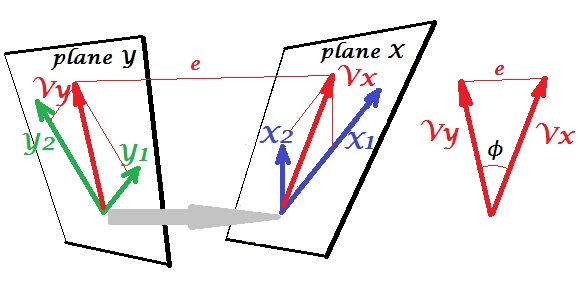
\includegraphics[width=0.7\textwidth]{Image/geometry.jpg}
    \caption{Geometric interpretation of CCA. The datasets $X$ and $Y$ span two separate 
    subspaces (planes). The canonical variates $\mathbf{V}_X$ and $\mathbf{V}_Y$ are the 
    directions within each plane that minimize the angle $\phi$ between them.}
    \label{fig:geometric_cca}
\end{figure}

The key geometric insight of CCA is as follows. Rather than analyzing each dataset in 
isolation, CCA looks for the relationship \emph{between} the two subspaces. Specifically, 
it identifies the pair of directions — one in the subspace of $X$ and one in the subspace 
of $Y$ — such that the angle $\phi$ between them is minimized. The canonical correlation 
$\rho$ is then defined as the cosine of this angle:
\[
    \rho = \cos(\phi).
\]

Two subspaces are said to be \emph{maximally correlated} when they are parallel, i.e., 
when the angle between them equals zero ($\phi = 0$, so $\rho = 1$). In this case, the 
two linear combinations $U = \mathbf{V}_X^\top X$ and $V = \mathbf{V}_Y^\top Y$ point 
in the same direction, indicating a perfect linear relationship between the two datasets. 
Conversely, when the subspaces are orthogonal ($\phi = 90^\circ$, $\rho = 0$), the datasets 
are uncorrelated.

The line $e$ in the figure represents the residual — the component that remains after 
projecting one canonical variate onto the other. Minimizing $e$ is equivalent to 
maximizing the canonical correlation $\rho$, which is precisely the objective of CCA.

In summary, CCA can be interpreted geometrically as finding the \emph{closest pair of 
directions} between two subspaces, where closeness is measured by the angle between them.